\documentclass{beamer}%

\usepackage[frenchb]{babel}%
\usepackage[T1]{fontenc}%
\usepackage[utf8]{inputenc}%

\usetheme{Warsaw}%

\usepackage{url}%
\usepackage{graphicx}%
\usepackage{listings}%

\usepackage[font=scriptsize]{caption}%
\usepackage{subfig}%

\usepackage{etoolbox}
\usepackage{ragged2e}%

\title{Projet 1: Pavage de Penrose et Tours de Hanoi}%
\author{Marco Freire, Clément Legrand-Duchesne}%
\institute{ENS de Rennes, Département Informatique 1A}%
\date{29 septembre 2017}%

%justifies all text appearing on every frame
\apptocmd{\frame}{}{\justifying}{}%

\begin{document}

	%prevents header from appearing on titlepage
	\begingroup 
		\setbeamertemplate{headline}{}
		\begin{frame}
			\titlepage
		\end{frame}
	\endgroup
	
	%prevents header from appearing on table of contents and displays
	%plan as frame title	
	\begingroup 
		\setbeamertemplate{headline}{}
		\addtobeamertemplate{frametitle}{\vspace*{-\headheight}}{}
		\begin{frame}{Plan}
			\tableofcontents
		\end{frame}
	\endgroup

	\section{Pavage de Penrose}
		\subsection{Principe}
			\begin{frame}
				\frametitle{Principe du pavage}
				\begin{figure}
					\centering
					\setcounter{subfigure}{0}
					\subfloat[Triangle d'or aigu]{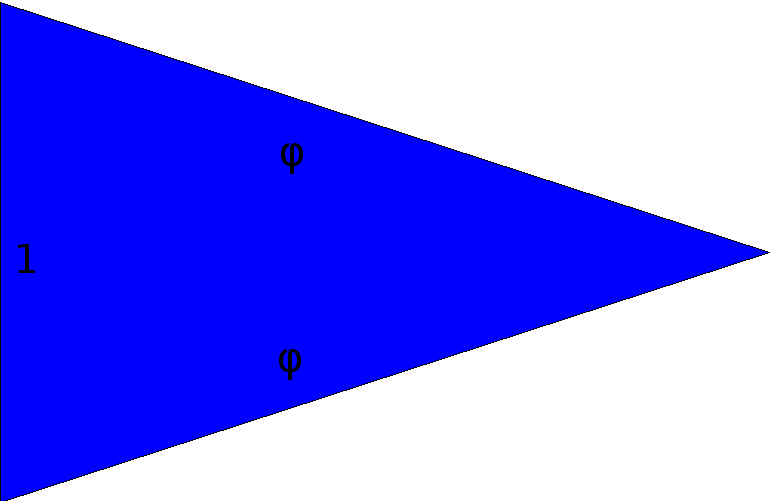
\includegraphics[width=5cm]{penrose_Acute_0.png}}\qquad
					\subfloat[Découpe en trois
                                        triangles d'or]{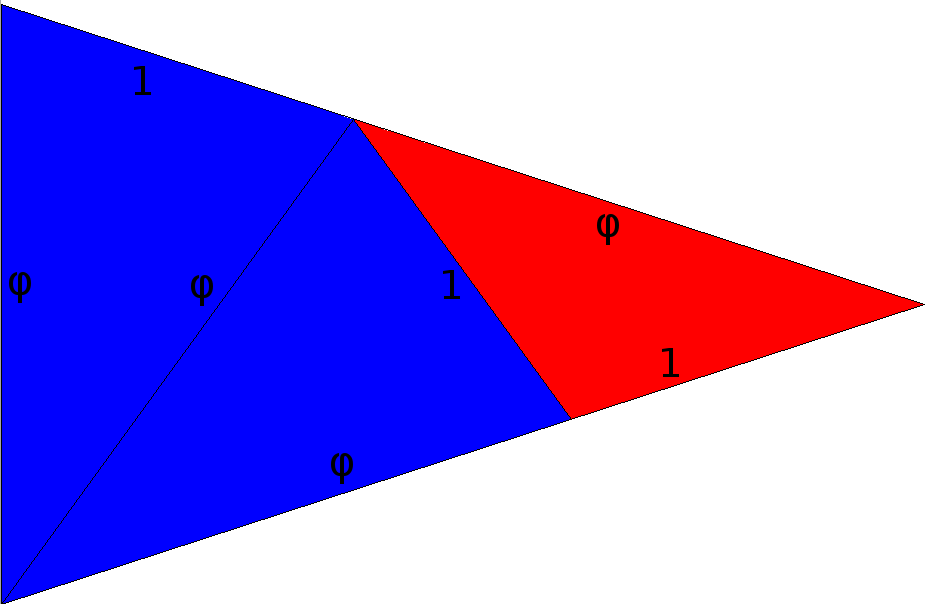
\includegraphics[width=5cm]{penrose_Acute_1.png}}
				\end{figure}	
				\begin{figure}
					\centering
					\subfloat[Triangle d'or obtus]{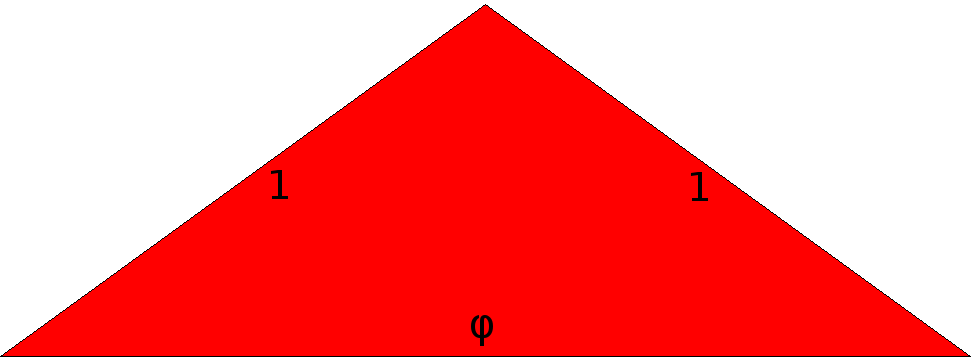
\includegraphics[width=5cm]{penrose_Obtuse_0.png}}\qquad
					\subfloat[Découpe en deux
                                        triangles d'or]{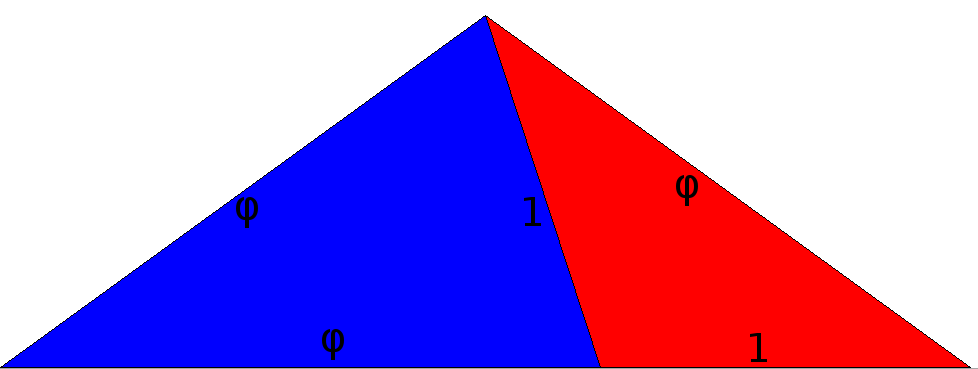
\includegraphics[width=5cm]{penrose_Obtuse_1.png}}
				\end{figure}
                         \end{frame}		
		
		\subsection{Implémentation}
			\begin{frame}
				\frametitle{Un premier algorithme}
                                Découpe récursive en partant d'un
                                grand triangle initial.
                                \begin{figure}
                                        \centering
                                        \subfloat[Éxécution de l'algorithme]{\includegraphics<1>[width=8cm]{anim0.pdf}}
                                        %\subfloat[Éxécution de l'algorithme]{\includegraphics<2>[width=8cm]{anim1.pdf}}
                                        %\subfloat[Éxécution de l'algorithme]{\includegraphics<3>[width=8cm]{anim2.pdf}}
                                        %\subfloat[Éxécution de l'algorithme]{\includegraphics<4>[width=8cm]{anim3.pdf}}
                                        %\subfloat[Éxécution de l'algorithme]{\includegraphics<5>[width=8cm]{anim4.pdf}}
                                \end{figure}
			\end{frame}
			
		\subsection{Améliorations}
			\begin{frame}
				EMPTY FRAME
			\end{frame}
			
	\section{Tours de Hanoi}
		\subsection{Principe}
		
			\begin{frame}
				\frametitle{Principe du jeu}
				\begin{figure}
					\centering
					\subfloat[État initial]{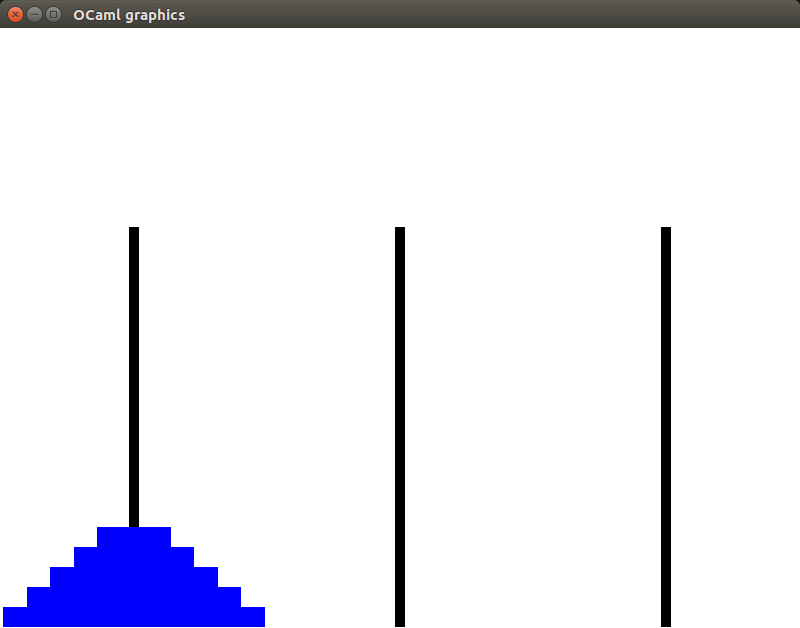
\includegraphics[width=5cm]{hanoi_start.png}}\qquad
					\subfloat[État final]{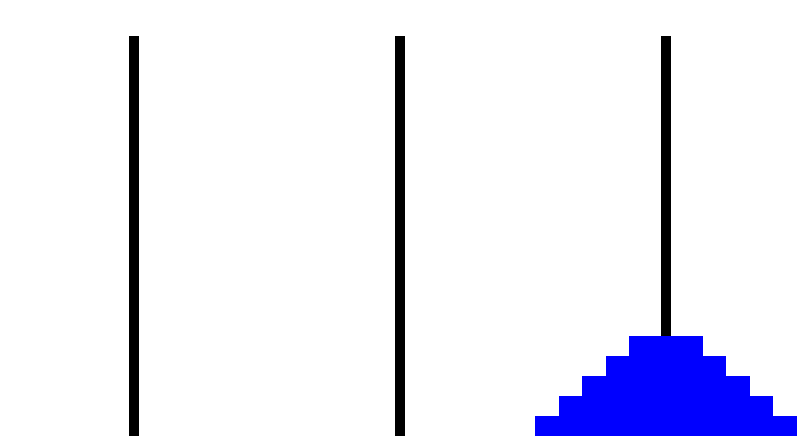
\includegraphics[width=5cm]{hanoi_end.png}}
				\end{figure}
				
				Le joueur doit déplacer les n disques initiaux du premier piquet au dernier
				en réalisant un seul mouvement à la fois, et avec la contrainte suivante:
				aucun disque ne peut être empilé à aucun moment sur un disque de taille inférieure.				
			\end{frame}
		
			\begin{frame}
				\frametitle{Algorithme simple}
				\begin{figure}
					\centering
					\setcounter{subfigure}{0}
					\subfloat[État initial]{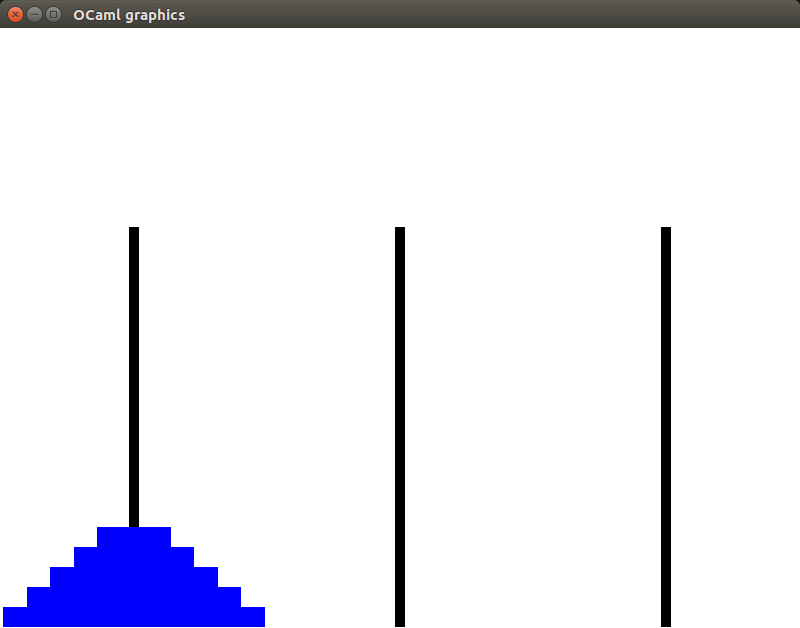
\includegraphics[width=5cm]{hanoi_start.png}}\qquad
					\subfloat[Étape 1]{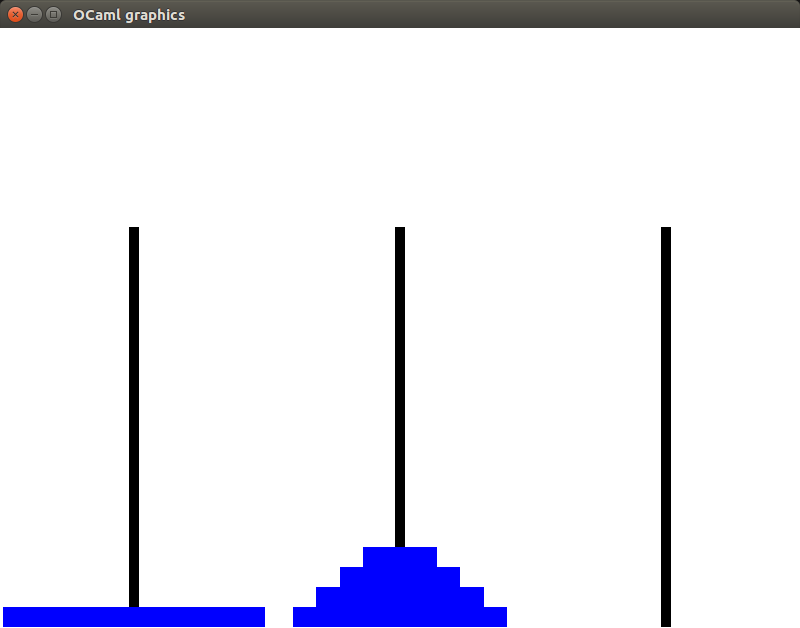
\includegraphics[width=5cm]{hanoi_mid1.png}}
				\end{figure}	
				\begin{figure}
					\centering
					\subfloat[Étape 2]{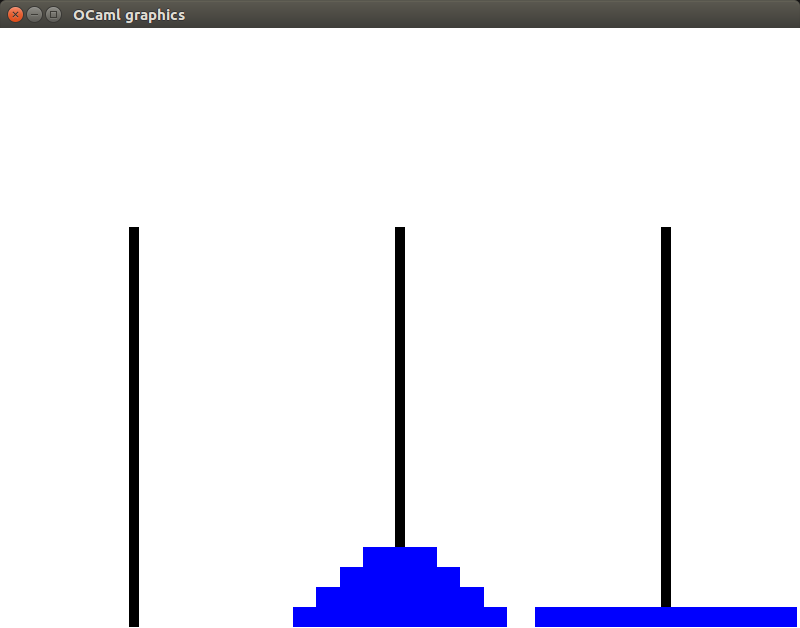
\includegraphics[width=5cm]{hanoi_mid2.png}}\qquad
					\subfloat[État final]{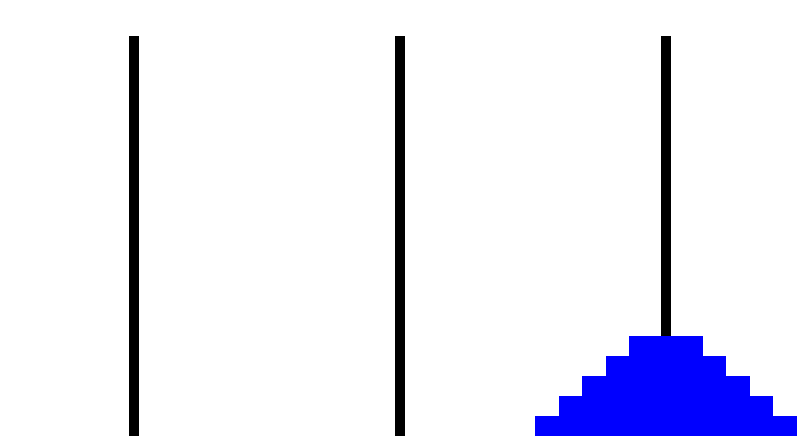
\includegraphics[width=5cm]{hanoi_end.png}}
				\end{figure}
			\end{frame}
			
			\begin{frame}
				\frametitle{Calcul du nombre de déplacements}
				\begin{description}
					\item[Initialisation] $M(0) = 1$
					\item[Relation de récurrence] $M(n) = 2M(n-1) + 1$
					\item[Relation générale] $M(n) = 2^n - 1$
				\end{description}
			\end{frame}
			
			\begin{frame}
				\frametitle{Algorithme généralisé}
				\begin{figure}
					\centering
					%resets figure numbering
					\setcounter{subfigure}{0}
					\subfloat[État initial]{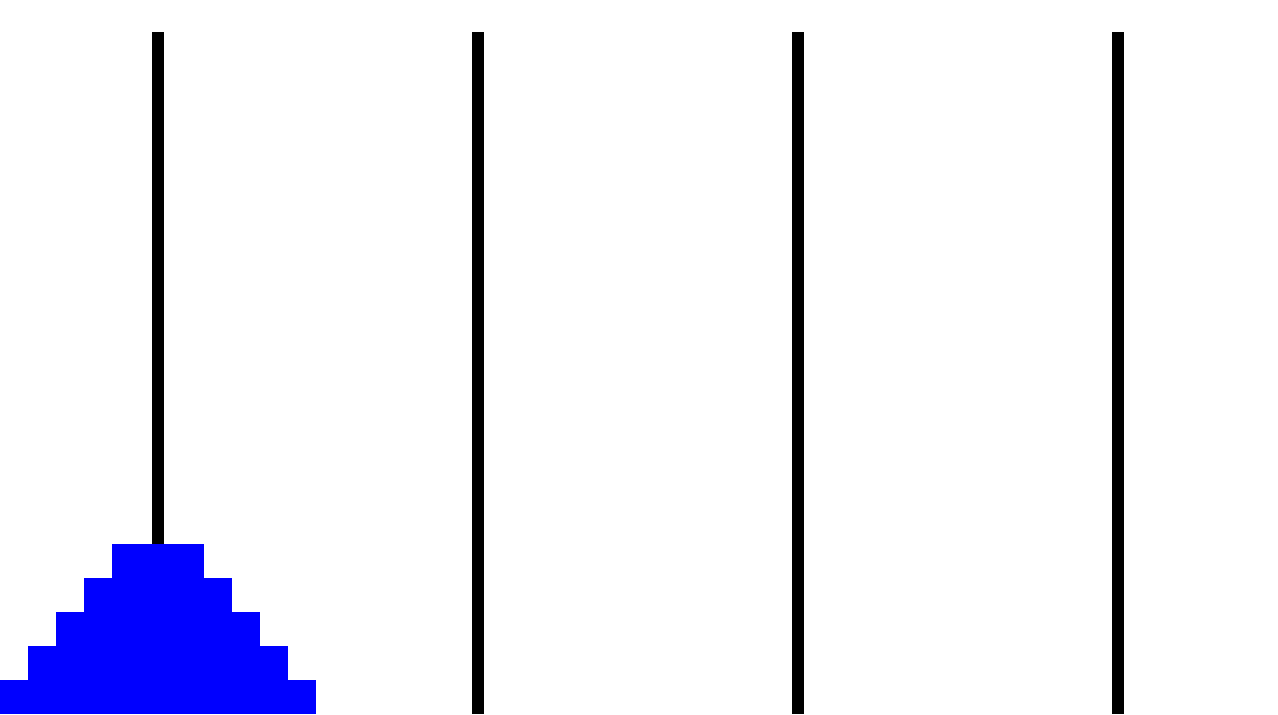
\includegraphics[width=5cm]{hanoi_gen_start.png}}\qquad
					\subfloat[Étape 1]{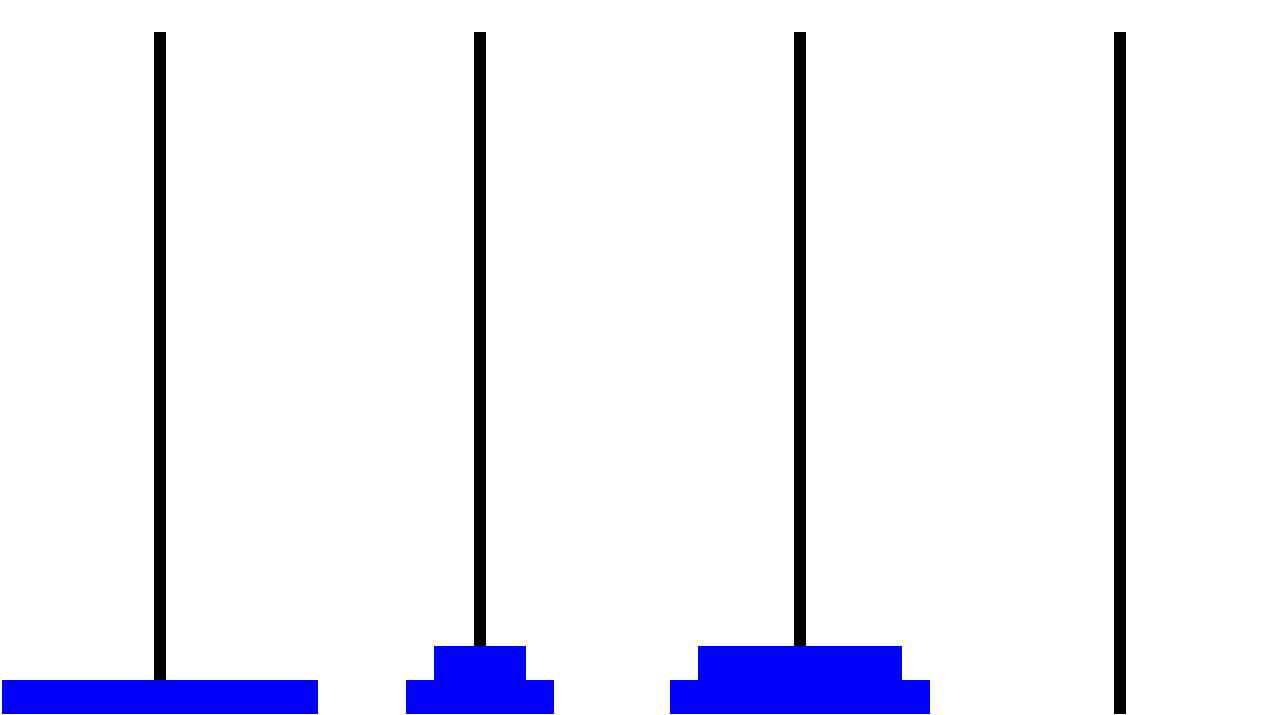
\includegraphics[width=5cm]{hanoi_gen_mid1.png}}
				\end{figure}	
				\begin{figure}
					\centering
					\subfloat[Étape 2]{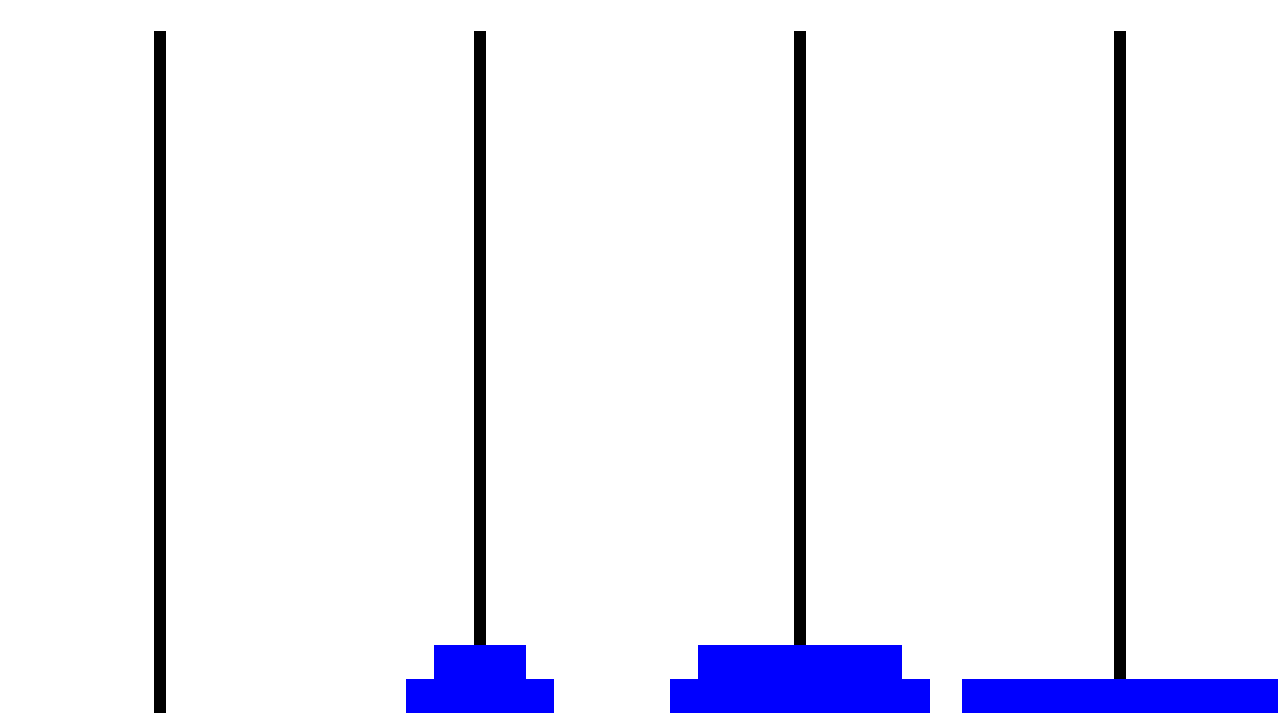
\includegraphics[width=5cm]{hanoi_gen_mid2.png}}\qquad
					\subfloat[État final]{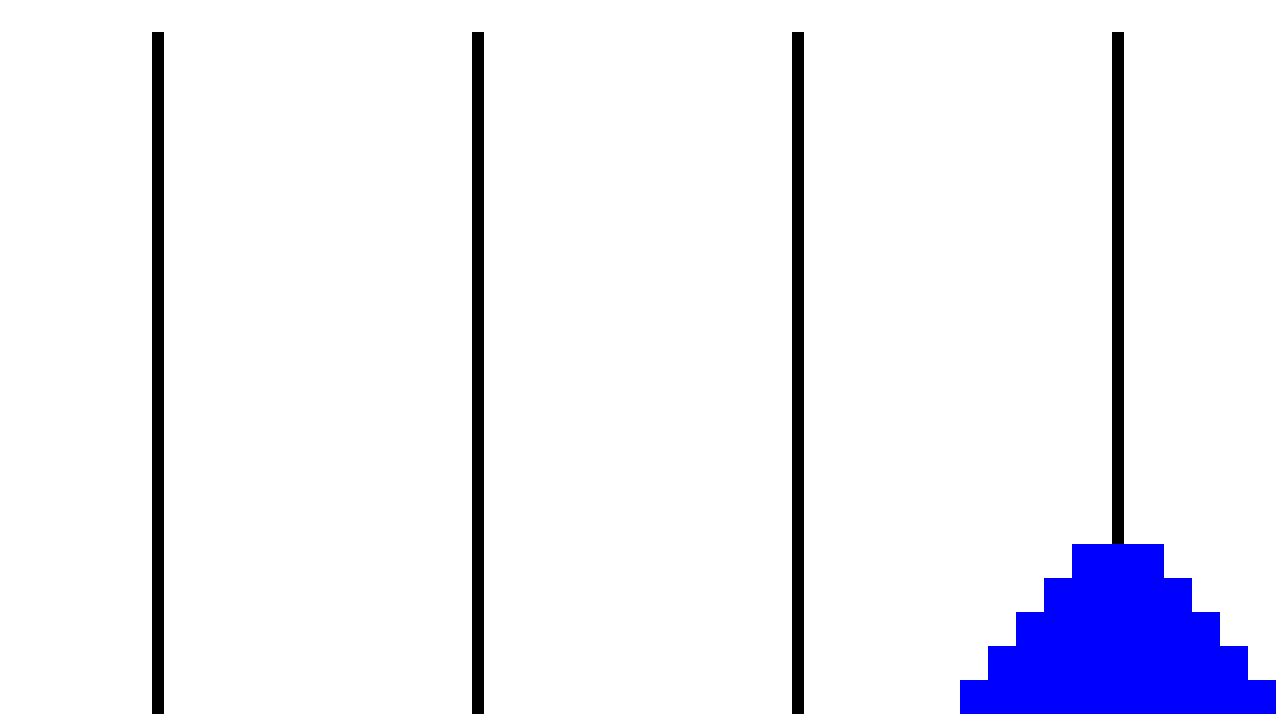
\includegraphics[width=5cm]{hanoi_gen_end.png}}
				\end{figure}
			\end{frame}
			
		\subsection{Implémentation}
			\begin{frame}
				\frametitle{Choix et extensions}
				La situation globale est représentée par un tableau de piles.
				\bigbreak
				Extensions créées:
				\begin{itemize}
					\item affichage graphique;
					\item généralisation du problème à n piquets.
				\end{itemize}
			\end{frame}
			
			\begin{frame}
				\frametitle{Problèmes rencontrés}
				Différents problèmes:
				\begin{enumerate}
					\item premier algorithme non-généralisable;
					\item généralisation de l'affichage.
				\end{enumerate}
			\end{frame}
			
		\subsection{Améliorations}
			\begin{frame}
				\frametitle{Algorithme simple}
				Le nombre de déplacements de disques effectués pas l'algorithme
				dans le cas où il n'y a que trois piquets est optimal.
				
				\begin{figure}
					\centering
					\subfloat{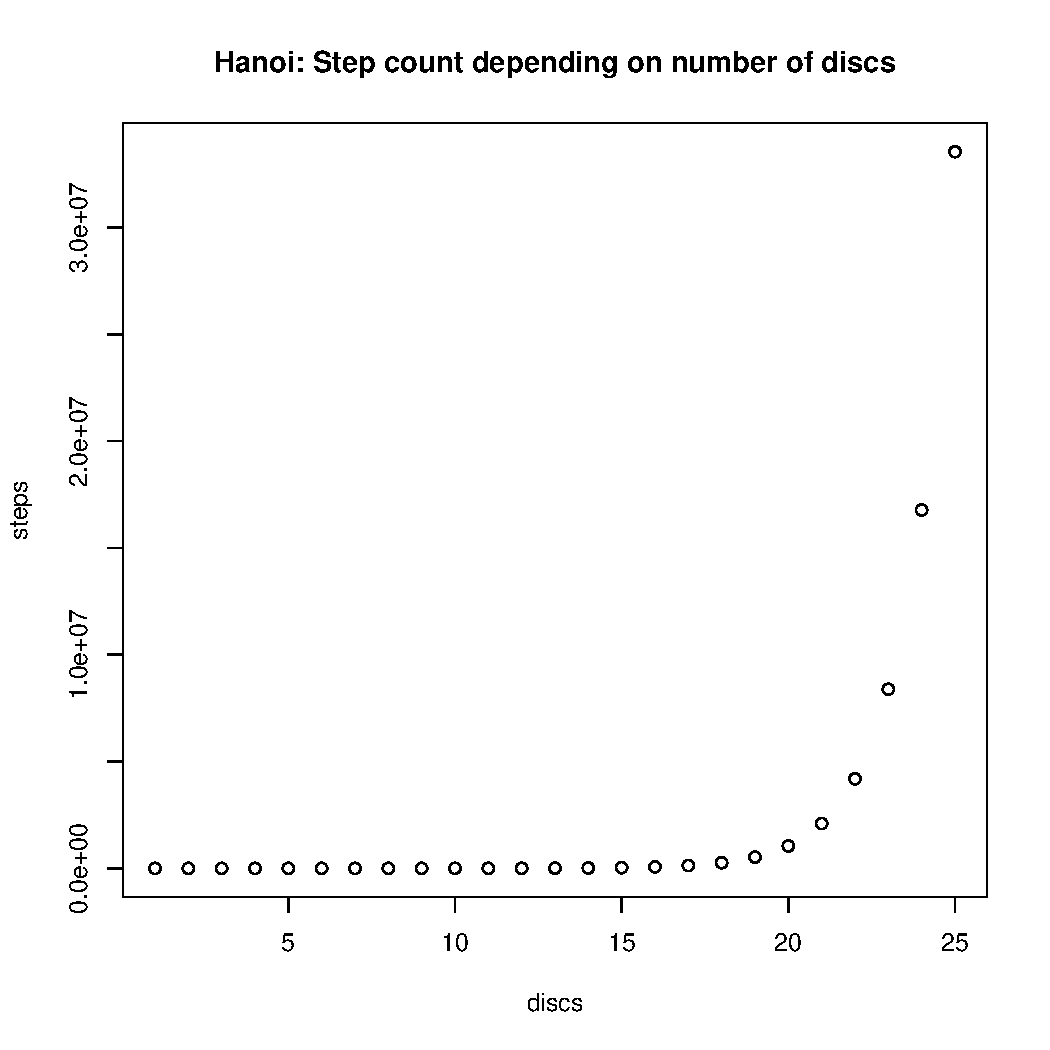
\includegraphics[width=.35\linewidth]{steps_plot.pdf}}\qquad
					\subfloat{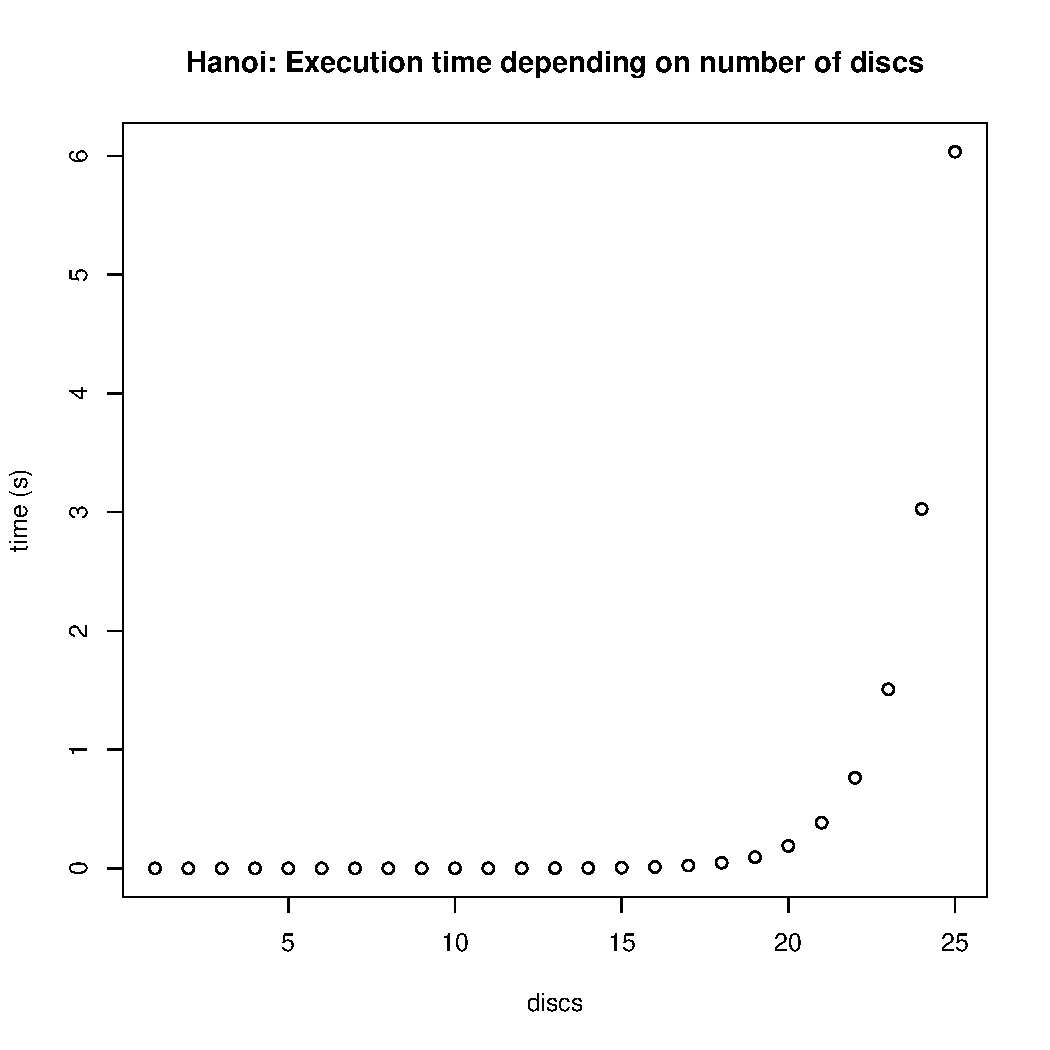
\includegraphics[width=.35\linewidth]{time_plot.pdf}}
				\end{figure}
				
				Les résultats expérimentaux sont en accord avec
				le calcul théorique:le nombre de mouvements
				le temps d'exécution sont fonction exponentielle du nombre
				initial de disques
			\end{frame}
			
			\begin{frame}
				\frametitle{Algorithme généralisé}
				À ce jour, la solution optimale des Tours de Hanoi à plus de quatre
				piquets est un problème ouvert.
				
				L'algorithme ici utilisé n'utilise pas la totalité de piquets libres.
				
				\begin{figure}
					\centering
					\setcounter{subfigure}{0}
					\subfloat[État 1]{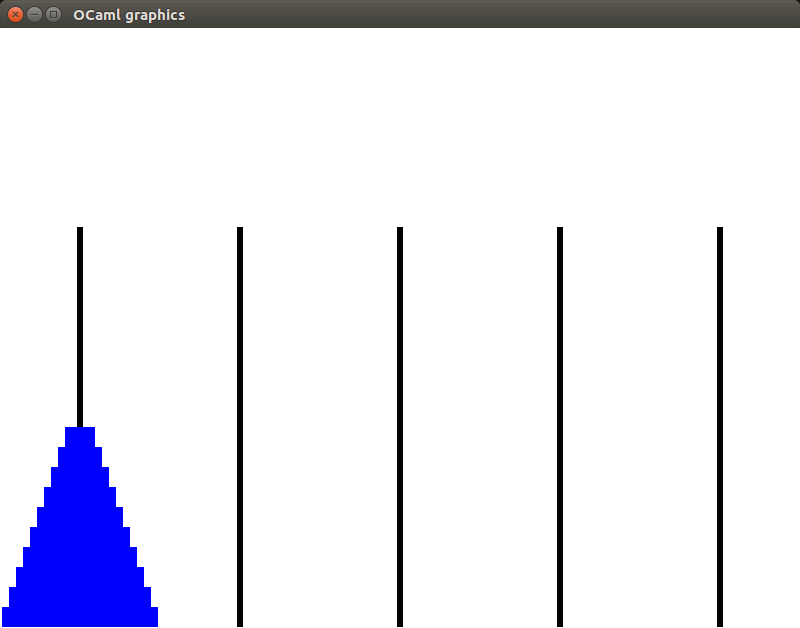
\includegraphics[width=.35\linewidth]{hanoi_pb_1.png}}\qquad
					\subfloat[État 2]{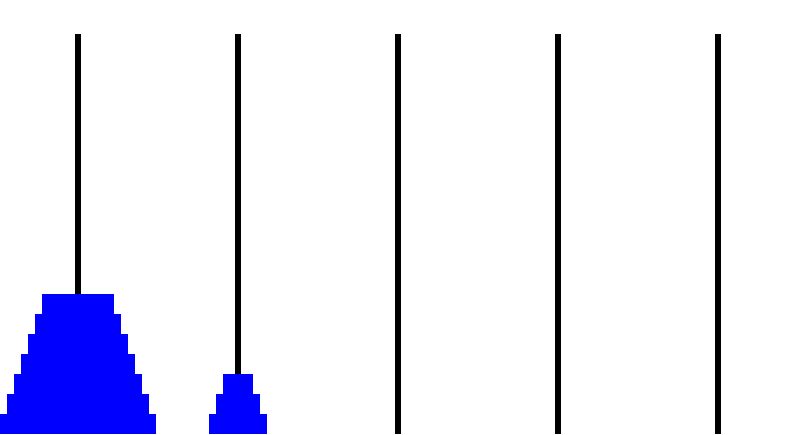
\includegraphics[width=.35\linewidth]{hanoi_pb_2.png}}
				\end{figure}
				
				Dans cette situation, pour passer d'un état à l'autre, uniquement le dernier
				piquet est utilisé pour stocker des disques, alors que les autres pourraient
				être utilisés de façon à effectuer moins de mouvements.
			\end{frame}
			
\end{document}
